\section{Design}
In questa sezione viene presentato il design del progetto, partendo dalle decisioni prese in ambito architetturale e proseguendo con il design di dettaglio.

\subsection{Design Architetturale}
Come illustrato nei capitoli precedenti, il progetto si propone di sviluppare un meccanismo per la creazione di sistemi multi-agente distribuiti utilizzando \textit{JaKtA}.
Il team ha deciso di raggiungere questo obiettivo fornendo un'estensione del \textit{framework} e del suo \textit{Domain Specific Language} il più minimale possibile.
Dal punto di vista architetturale, il progetto si colloca come modulo a sé stante, come mostrato nella figura \ref{fig:architecture}:

\begin{figure}[ht!]
    \centering
    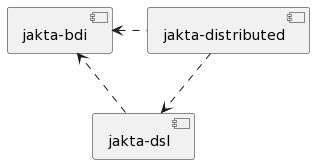
\includegraphics[width=0.8\textwidth]{figures/general-architecture.png}
    \caption{Architettura del progetto}
    \label{fig:architecture}
\end{figure}

In particolare, il modulo sviluppato è formato da tre componenti principali, come mostrato nella figura \ref{fig:detailed-architecture}:

\begin{figure}[ht!]
    \centering
    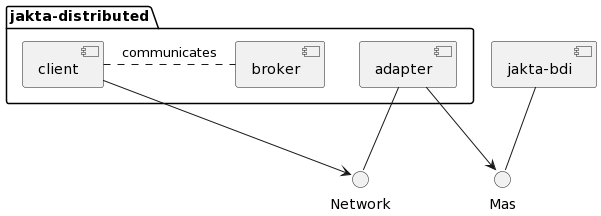
\includegraphics[width=0.8\textwidth]{figures/detailed-architecture.png}
    \caption{Architettura del modulo sviluppato}
    \label{fig:detailed-architecture}
\end{figure}

Dei moduli rappresentati in figura \ref{fig:detailed-architecture}, il modulo \textit{Adapter} è quello che definisce e contiene tutti i concetti da implementare per realizzare l'obiettivo di progetto,
mentre i moduli \textit{Client} e \textit{Broker} forniscono una prima implementazione della logica di comunicazione tra i sistemi multi-agente distribuiti.\\

Come anticipato in precedenza, il progetto presenta anche un'estensione del \textit{Domain Specific Language} di JaKtA, la cui struttura è rappresentata nella figura \ref{fig:dsl-architecture}.

\begin{figure}[ht!]
    \centering
    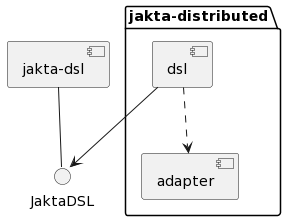
\includegraphics[width=0.8\textwidth]{figures/dsl-architecture.png}
    \caption{Architettura del Domain Specific Language}
    \label{fig:dsl-architecture}
\end{figure}

\subsubsection{Architettura di Rete}

Il diagramma dei componenti presentato in Figura \ref{fig:network-architecture} offre una panoramica dell'architettura di rete.
Il \textit{Broker} espone quattro interfacce: le interfacce \texttt{/subscribe/{topic}} e \texttt{/publish/{topic}} consentono rispettivamente la sottoscrizione e la pubblicazione su \textit{topic} specifici, mentre l'interfaccia \texttt{/topics} permette di recuperare l'elenco dei \textit{topic} disponibili. Inoltre, l'interfaccia \texttt{/subscribe-all/\{except...\}} offre la possibilità di sottoscrivere a tutti i \textit{topic} tranne quelli specificati. Il \textit{MAS}, d'altra parte, si connette al \textit{Broker} attraverso queste interfacce, sfruttandole per sottoscrivere, pubblicare e ottenere informazioni dagli altri \textit{MAS}. Questo setup permette la gestione delle comunicazioni distribuite, con il \textit{Broker} che funge da fulcro centrale per agevolare la sottoscrizione, la pubblicazione e la gestione dei \textit{topic} all'interno del sistema.

\begin{figure}[ht!]
    \centering
    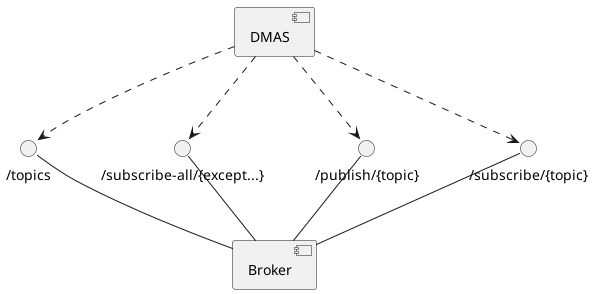
\includegraphics[width=0.8\textwidth]{figures/network-architecture.png}
    \caption{Architettura di rete}
    \label{fig:network-architecture}
\end{figure}

\subsection{Design di Dettaglio}
Nel progettare un'estensione del \textit{framework} che permetta la comunicazione tra sistemi multi-agente distribuiti, è importante stabilire cosa viene condiviso tra questi sistemi.
A tal proposito ci sono diverse possibilità da considerare:
\begin{itemize}
    \item Condividere l'\textit{Environment}: in questo caso, gli agenti di ogni sistema multi-agente operano nello stesso \textit{Environment}. Questa soluzione è stata ritenuta complessa e rischiosa da implementare,
    poiché l'\textit{Environment} è una struttura dati complessa e cruciale per il funzionamento del sistema multi-agente, e la sua condivisione tra più sistemi richiederebbe una gestione molto robusta della consistenza dei dati tra i vari sistemi;
    \item Condividere gli agenti: in questo caso, sistemi multi-agente diversi possono condividere agenti. Questa soluzione è un sottoinsieme della precedente, ma presenta gli stessi problemi;
    \item Condividere i messaggi tra gli agenti: in questo caso, sistemi multi-agente diversi possiedono \textit{Environment} ed agenti diversi, ma gli agenti di un sistema possono inviare messaggi agli agenti di un altro sistema.
\end{itemize}

Il team ha ritenuto l'ultima soluzione la più semplice ed efficace da implementare, in quanto la condivisione di un messaggio non presenta le stesse criticità dell'implementazione di strutture dati condivise. Inoltre si ritiene che questa soluzione offra comunque grande flessibilità e possibilità di realizzare comportamenti complessi tra i vari sistemi multi-agente.

La soluzione proposta consiste dunque nell'implementazione di una versione alternativa dell'interfaccia \texttt{Mas}, chiamata \texttt{Dmas}, da utilizzare in contesti distribuiti.
Questa estensione dovrà comportarsi come un \texttt{Mas}, ma in aggiunta dovrà essere in grado di comunicare con altri \texttt{Dmas} attraverso la rete.

\subsubsection{Adapter}
Questo modulo si occupa di definire i concetti di:

\begin{itemize}
    \item \textbf{Dmas}: rappresenta un sistema multi-agente distribuito, cioè che può comunicare con altri sistemi \texttt{Dmas} attraverso la rete.
    \item \textbf{Network}: incapsula la logica di comunicazione tra \texttt{Dmas} attraverso la rete.
    \item \textbf{RemoteService}: rappresenta un agente remoto, cioè un agente che appartiene ad un \texttt{Dmas} diverso da quello corrente, ma raggiungibile attraverso la rete.
\end{itemize}

Le relazioni tra questi concetti sono esemplificate dal diagramma delle classi in figura \ref{fig:class-dmas}.

\begin{figure}[ht!]
    \centering
    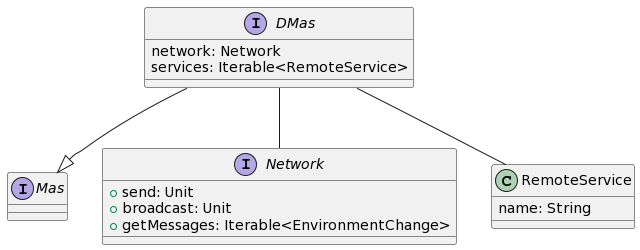
\includegraphics[width=0.8\textwidth]{figures/class-dmas.png}
    \caption{Diagramma delle classi del modulo Adapter}
    \label{fig:class-dmas}
\end{figure}

\subsubsection{Broker}

Il diagramma delle classi del \textit{broker} (Figura \ref{fig:broker-class-diagram}) presenta una struttura organizzata e modulare. Nel package \texttt{model}, sono definite due interfacce chiave: \texttt{Cache<T>} per la registrazione, la liberazione e la lettura di dati associati a un \textit{topic}, e \texttt{SubscriptionManager<T>} per gestire la sottoscrizione, l'aggiunta e la rimozione di \textit{publisher} e \textit{subscriber}, nonché l'ottenimento dei \textit{topic} disponibili e dei \textit{subscriber} associati a un \textit{topic}. Il package \texttt{plugins} include le classi \texttt{Routing} e \texttt{Websockets}, che vengono utilizzate per la definizione delle \textit{API Web}

\begin{figure}[ht!]
    \centering
    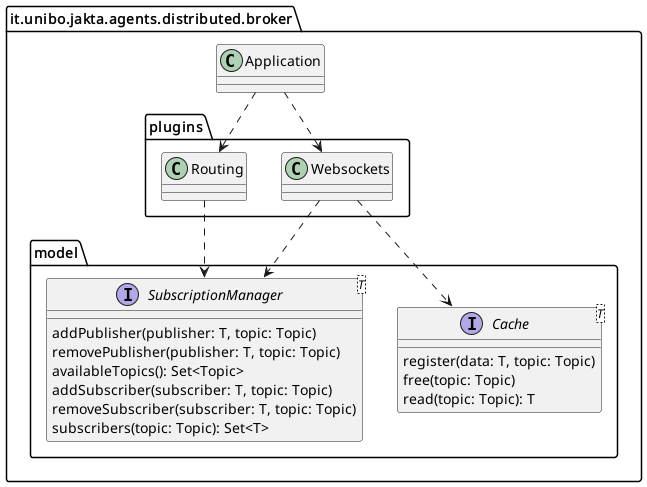
\includegraphics[width=0.8\textwidth]{figures/broker-class-diagram.png}
    \caption{Diagramma delle classi del \textit{Broker}}
    \label{fig:broker-class-diagram}
\end{figure}

\subsection{Comportamento}
Il comportamento delle varie componenti del sistema può essere descritto attraverso i seguenti passaggi.

\subsubsection{Inizializzazione del Sistema}

\begin{enumerate}
    \item istanziazione di una \texttt{Network};
    \item connessione da parte della \texttt{Network} al \textit{broker};
    \item definizione dei \texttt{RemoteService} di interesse;
    \item istanziazione di un \texttt{Dmas};
    \item per ogni \texttt{RemoteService}, il \texttt{Dmas} si sottoscrive ai \textit{topic} di interesse;
    \item esecuzione del dispatch della \texttt{ExecutionStrategy} scelta per il \texttt{Dmas};
\end{enumerate}

Queste attività sono illustrate in figura \ref{fig:initialization}.

\begin{figure}
    \centering
    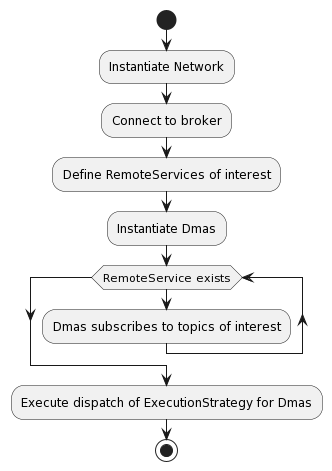
\includegraphics[width=0.8\textwidth]{figures/activity-dmas.png}
    \caption{Inizializzazione del sistema}
    \label{fig:initialization}
\end{figure}

\subsubsection{Ciclo di Esecuzione del Dmas}

\begin{enumerate}
    \item il \texttt{Dmas} raccoglie tutti gli eventi esterni ricevuti dalla \texttt{Network}, ossia i messaggi pubblicati dai \texttt{RemoteService} a cui si è sottoscritto e le eventuali notifiche di disconnessione di un \texttt{RemoteService}, sotto forma di \texttt{EnvironmentChange};
    \item gli eventi esterni vengono concatenati alla coda degli \texttt{EnvironmentChange} interni del \texttt{Dmas};
    \item ad uno ad uno, gli \texttt{EnvironmentChange} vengono processati dal \texttt{Dmas}. Nel caso in cui l'evento consista nell'inviare un messaggio ad un \texttt{RemoteService} o un \textit{broadcast}, il messaggio viene inviato alla \texttt{Network}, che si occuperà di inoltrarlo al \textit{broker};
\end{enumerate}

Queste attività sono illustrate in figura \ref{fig:execution}.

\begin{figure}
    \centering
    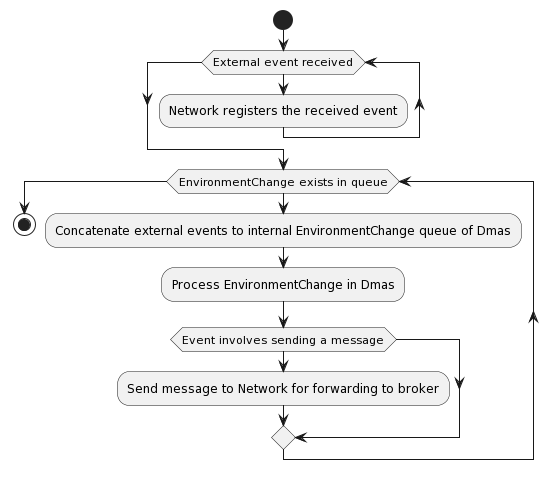
\includegraphics[width=0.8\textwidth]{figures/activity-applychanges.png}
    \caption{Ciclo di esecuzione del \texttt{Dmas}}
    \label{fig:execution}
\end{figure}

\subsection{Interazioni}
Il modello di interazione tra i vari \texttt{Dmas} collegati alla rete è di tipo \textit{publish-subscribe}: ogni \texttt{Dmas}, che assume il ruolo di \textit{client}, può sottoscrivere ad uno o più \textit{topic}, e può pubblicare messaggi su uno o più \textit{topic}.
I messaggi pubblicati su un \textit{topic} vengono ricevuti da tutti i \textit{client} che si sono sottoscritti a quel \textit{topic}.
Il \textit{broker}, che assume il ruolo di server, si occupa di gestire la comunicazione tra i \textit{client}, in particolare si occupa di:
\begin{itemize}
    \item ricevere i messaggi pubblicati dai \textit{client};
    \item inviare i messaggi ai \textit{client} sottoscritti ai \textit{topic} corrispondenti;
    \item gestire le connessioni e le disconnessioni dei \textit{client}.
    \item gestire la sottoscrizione dei \textit{client} ai vari \textit{topic}.
\end{itemize}

Il comportamento di \textit{client} e \textit{broker} in situazioni di \textit{broadcast} e invio di messaggi con singolo destinatario è illustrato nelle figure \ref{fig:interaction-broadcast} e \ref{fig:interaction-sendmessage}.

\begin{figure}[ht!]
    \centering
    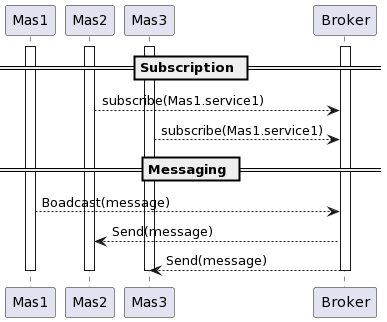
\includegraphics[width=0.8\textwidth]{figures/interaction-broadcast.png}
    \caption{Interazione tra \texttt{Dmas}, \textit{client} e \textit{broker} in caso di \textit{broadcast}}
    \label{fig:interaction-broadcast}
\end{figure}

\begin{figure}[ht!]
    \centering
    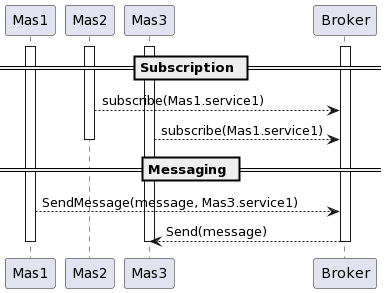
\includegraphics[width=0.8\textwidth]{figures/interaction-sendmessage.png}
    \caption{Interazione tra DMas, \textit{client} e \textit{broker} in caso di invio di messaggio con singolo destinatario}
    \label{fig:interaction-sendmessage}
\end{figure}

\subsubsection{Gestione delle disconnessioni}
Essendo il sistema distribuito, è importante assumere che possano avvenire delle disconnessioni di un qualsiasi partecipante al sistema, sia esso un \texttt{Dmas} o il \textit{broker}.
La strategia generale del sistema è quella di creare, a fronte di una disconnessione, un \texttt{EnvironmentChange} di tipo \texttt{SendMessage} per ogni agente dei \texttt{Dmas} sottoscritti al
partecipante disconnesso, in modo che questi possano essere informati della disconnessione e possano agire di conseguenza. È importante notare come questa strategia lasci il compito
di gestire i fallimenti al programmatore degli agenti del \texttt{Dmas}.

Nelle figure \ref{fig:interaction-disconnect} e \ref{fig:interaction-disconnect-broker} è possibile osservare come il sistema gestisce le disconnessioni di un \texttt{Dmas} e del \textit{broker}.

\begin{figure}[ht!]
    \centering
    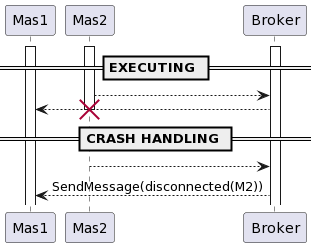
\includegraphics[width=0.8\textwidth]{figures/sequence-client-crash.png}
    \caption{Interazione tra \texttt{Dmas}, \textit{client} e \textit{broker} in caso di disconnessione di un \texttt{Dmas}}
    \label{fig:interaction-disconnect}
\end{figure}

\begin{figure}[ht!]
    \centering
    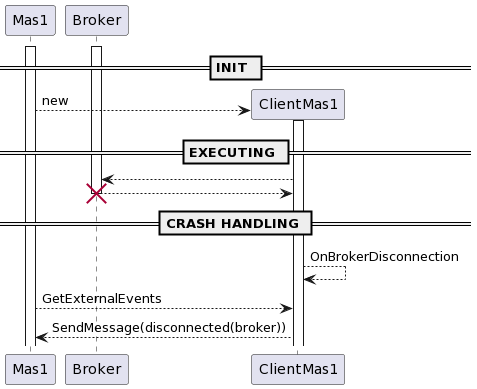
\includegraphics[width=0.8\textwidth]{figures/sequence-broker-crash.png}
    \caption{Interazione tra \texttt{Dmas}, \textit{client} e \textit{broker} in caso di disconnessione del \textit{broker}}
    \label{fig:interaction-disconnect-broker}
\end{figure}